\documentclass{article}
\usepackage[utf8]{inputenc}
\usepackage{subfig}
\usepackage{amsmath}

\usepackage{graphicx}
\usepackage[legalpaper, landscape, margin=0.5cm]{geometry}

\thispagestyle{empty}
% \renewcommand{\thesubfigure}{\roman{subfigure}}
\begin{document}

\begin{figure}[h]
        \centering
        \subfloat[horizontal cut]{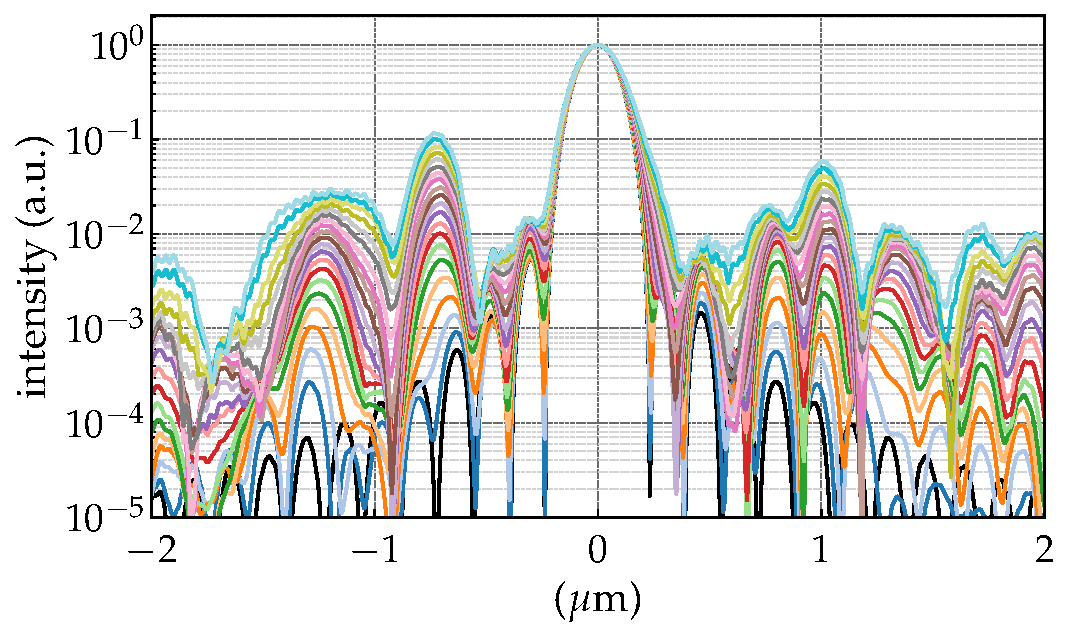
\includegraphics[height=3.3cm]{figures/ch05/hf_scan/SE_hf_X_scan.pdf}}\hspace{0.1cm}
        \subfloat[vertical cut]{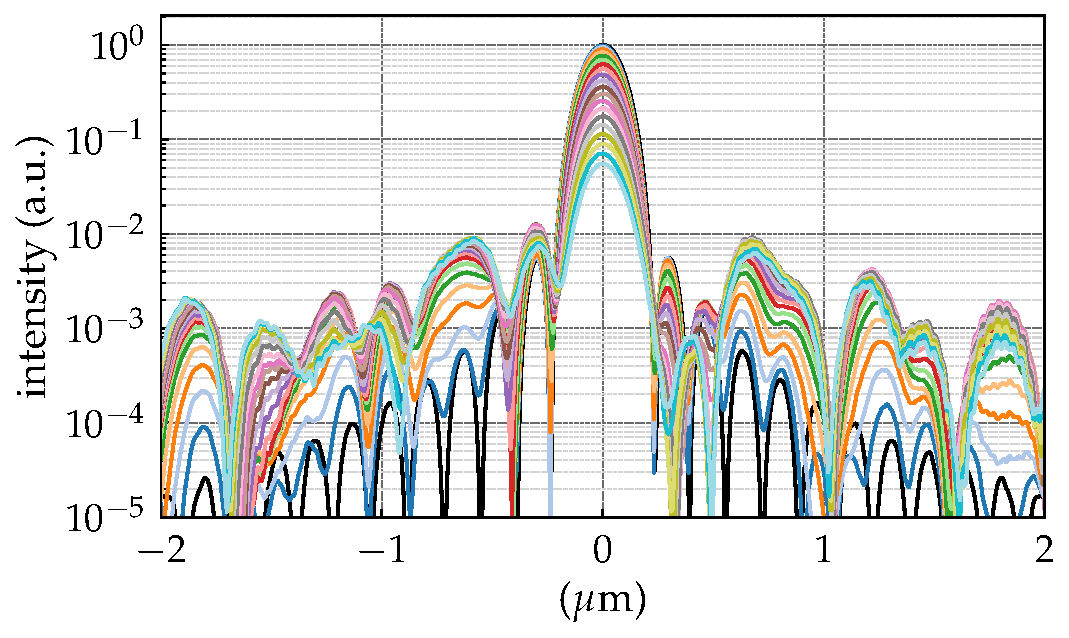
\includegraphics[height=3.3cm]{figures/ch05/hf_scan/SE_hf_Y_scan.pdf}}\hspace{0.1cm}
        \caption*{coherent simulations}
        
        \subfloat[horizontal cut]{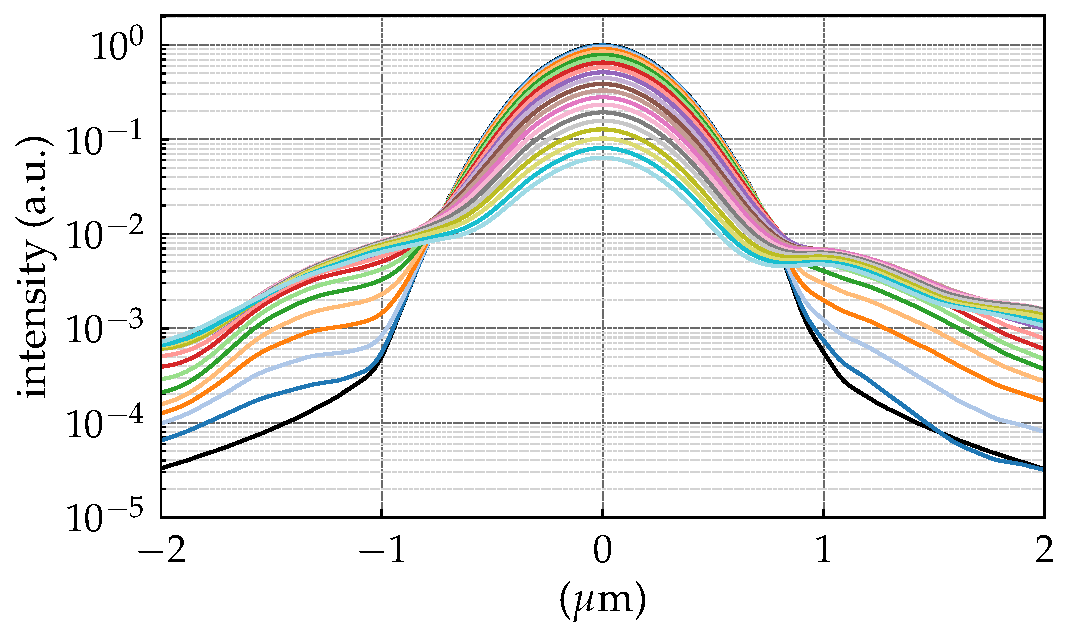
\includegraphics[height=3.3cm]{figures/ch05/hf_scan/ME_hf_X_cut_scan.pdf}}\hspace{0.1cm}
        \subfloat[vertical cut]{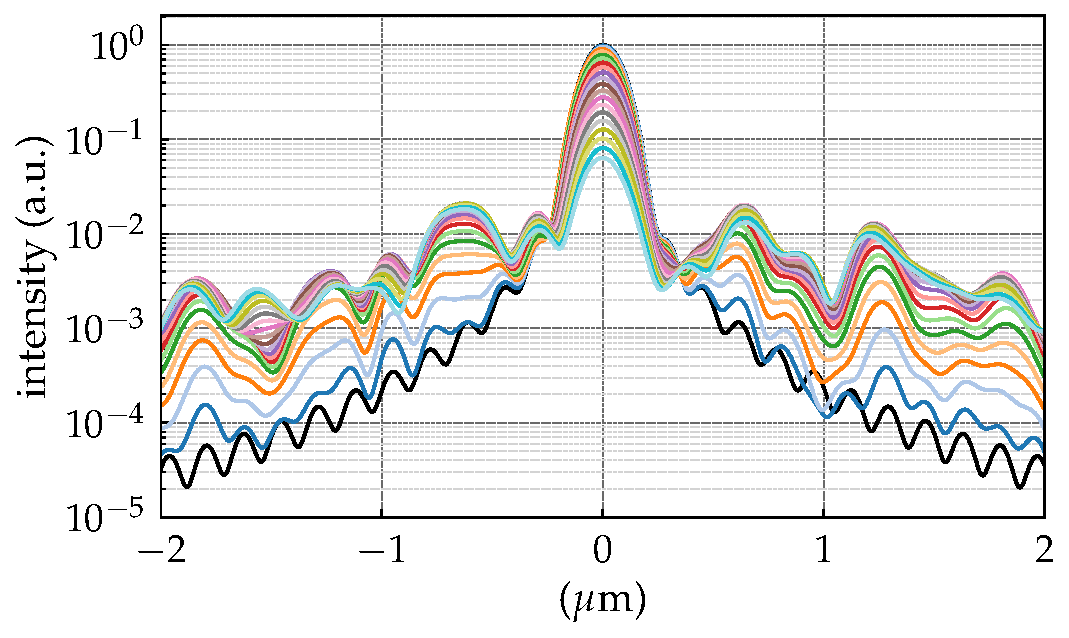
\includegraphics[height=3.3cm]{figures/ch05/hf_scan/ME_hf_Y_cut_scan.pdf}}\hspace{0.1cm}
        \caption*{partially-coherent simulations}

        \subfloat[figure error ($\mu$m)]{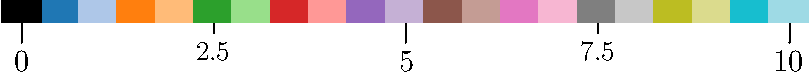
\includegraphics[height=0.7cm]{figures/ch05/hf_scan/graph_legend.pdf}}

\end{figure}
\end{document}